\documentclass[a4paper]{article}
\title{利用马尔可夫状态模型分析分子动力学模拟轨迹}                   %———总标题
   \author{王韬 2024221120}
	\date{2025 年 1 月 8 日}
\usepackage{subfigure}
\usepackage{graphicx}
\usepackage{float}
\usepackage{ctex}
\usepackage{CJKutf8}

\renewcommand{\abstractname}{\textbf{\zihao{4}摘要}}
\begin{document}
	
\begin{CJK}{UTF8}{gbsn}
\CJKfamily{song}
\maketitle

\begin{center}
\tableofcontents
\end{center}

\newpage

 \begin{abstract}

分子动力学模拟需要消耗较多的计算资源。在科学研究中,为了缩减计算所需要的时间,研究人员会使用多个计算机进行并行计算来代替在单个计算机上进行长时间计算。遗憾的是,并行计算所生成的轨迹并不能直接拼合成一条单独的长时间轨迹。面对这一困境,马尔可夫状态模型得到了广泛的应用。对于多个并行计算结果,可以提取构象的特征,并构建转移矩阵,从而解释长时间尺度的分子运动过程。丙氨酸二肽是很有代表性的小分子,它的二面角构象十分丰富,同时分子结构简单,适合用来研究分子动力学的运动过程。对丙氨酸二肽的模拟揭示了马尔可夫状态模型的可行性,这种方法可以推广到更复杂的蛋白之上,用以研究复杂蛋白的运动过程。

 \end{abstract}

\newpage


\section{介绍}
	\subsection{丙氨酸二肽}

	分子动力学研究中的丙氨酸二肽并不是简单的将两个丙氨酸残基以肽键连接起来,而是使用乙酰基和甲胺基封端,这样就排除了电荷影响。这是一个常用来研究蛋白质中氨基酸的构象行为的典型模型分子,其结构如下图所示。

\begin{figure}[H]
\centering
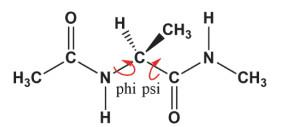
\includegraphics[scale=0.35]{ala_di.jpg}
\caption{丙氨酸二肽的结构}
\end{figure}

	从图中可以看出,丙氨酸二肽运动的最直接变化值就是二面角,后续也将以此为主要参照进行研究。


	
	\subsection{K-Medoids聚类}

K-Medoids算法在K-means算法的基础上衍生而来,K-Means聚类算法的目的是将分子动力学(MD)数据集划分为K个不重叠的聚类$\{C_{1},C_{2}, \cdots,  C_{k}\}$,使不同的状态与相应聚类中心(几何平均值)的距离平方和最小化。其算法可以表示为

\begin{equation}
min\sum_{i=1}^{K}\sum_{x\in C_{i}}^{} {\vert\vert x- \mu_{i} \vert\vert}^{2}
\end{equation}

其中,$x$为第$i$个聚类$C_{i}$中的MD构象,$\mu_{i}$为聚类中心。


这种方法可以对不同的MD数据进行聚类,生成“微状态”代表一部分轨迹。但这种方法的缺点在于生成的微状态并不一定是动力学过程中的一帧轨迹,原因在于K-Means方法对轨迹计算了平均值。在此,我使用K-Medoids算法进行聚类,这种方法与K-Means的区别在于K-Medoids的聚类中心选取了模拟的一帧轨迹,而非轨迹的均值,其算法可以表示为

\begin{equation}
min\sum_{i=1}^{K}\sum_{x\in C_{i}}^{} {\vert\vert x- \mathrm C(C_{i}) \vert\vert}^{2}
\end{equation}


其中,$\mathrm C(C_{i})$是作为聚类中心的构象,而非均值。


	\subsection{计算转移矩阵}
计算得到转移矩阵是构建马尔可夫过程十分重要的一个步骤,下图为分子动力学轨迹构建转移矩阵的示意图。

\begin{figure}[H]
\centering
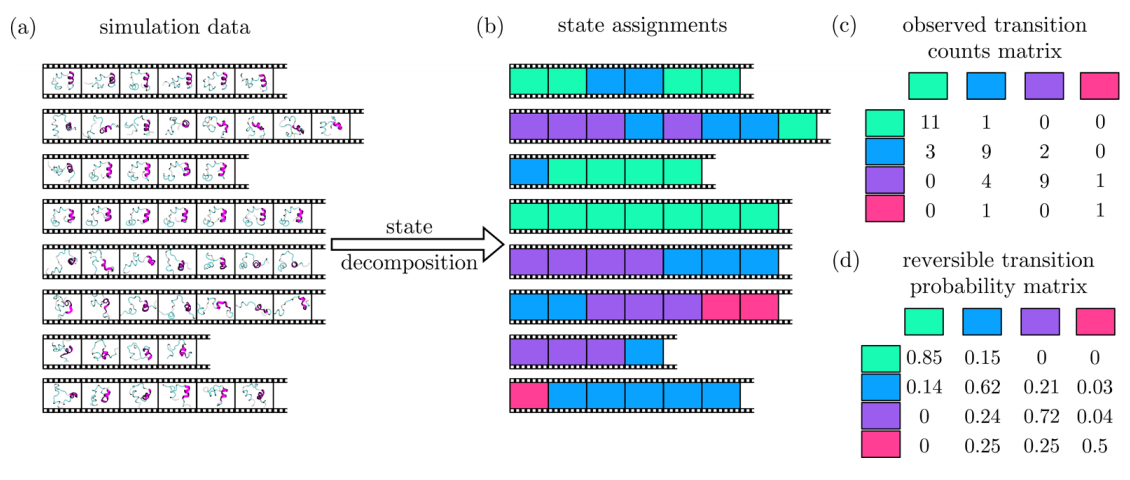
\includegraphics[scale=0.48]{trans_matrix.png}
\caption{转移矩阵示意图}
\end{figure}



	\subsection{验证马尔可夫状态模型}

验证模型可以通过观察隐含时间尺度$t_{i}$的收敛实现,伴随着$\tau$值的不断增大,$t_{i}$应该与马尔可夫系统中的$\tau$无关。在构建转移矩阵后,我们可以得到只有一行的“特征值”,其中数值更大的特征值表示该状态衰减更慢,对应到马尔可夫过程即为更长的时间尺度。更长的时间尺度代表着更慢、可能也是更重要的过程。因此此处选取了排名前十的特征值,并以$\tau$横坐标,$t_{i}$为纵坐标作图。$t_{i}$可以使用如下公式计算


\begin{equation}
t_{i} = -\frac{\tau}{log(\lambda_{i})}
\end{equation}

其中$\lambda_{i}$为特征值, $\tau$为采样一次的时间。





\section{结果}
	\subsection{丙氨酸二肽有6个自由能高值}
		已有的研究手动选择了六种状态,在这些状态下分子的能量较大,我使用该报道中的结果与模拟结果进行对比,证明了模拟的正确性,在我的模拟中,丙氨酸二肽运动轨迹的自由能景观图与已有报道相一致。这说明我的模拟结果是正确的,可以用于接下来的研究。

\begin{figure}[H]
\centering  
\subfigure[先验景观]{
\label{Fig.sub.1}
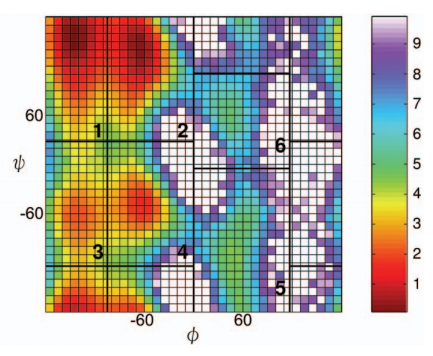
\includegraphics[width=0.35\textwidth]{tr_force.png}}
\subfigure[模拟景观]{
\label{Fig.sub.2}
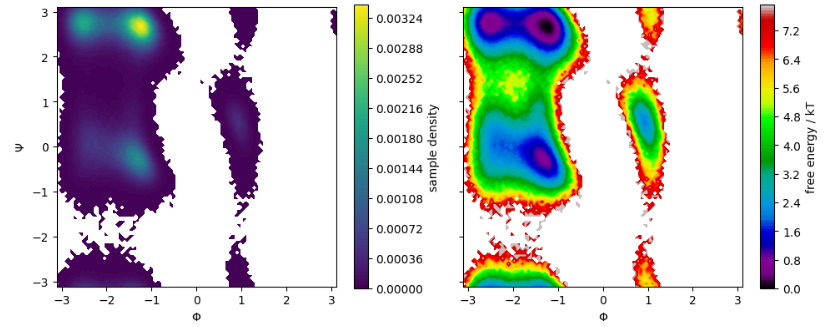
\includegraphics[width=0.65\textwidth]{free_energy.png}}
\caption{能量景观对比}
\label{Fig.main}
\end{figure}




	

	\subsection{马尔可夫模型描述丙氨酸二肽的运动可以收敛}

	首先对分子动力学模拟轨迹进行聚类,使用聚类结果构建转移矩阵,聚类结果如下图所示。
\begin{figure}[H]
\centering
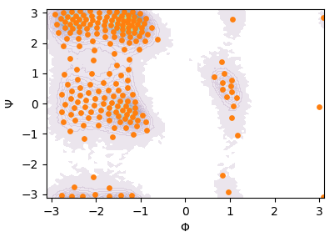
\includegraphics[scale=0.75]{clus.png}
\caption{聚类结果}
\end{figure}

	随后计算马尔可夫模型的隐含时间尺度,这是Chapman-Kolmogorov检验的简化版本。在这里我比较了不同数量的聚类中心对时间的影响,结果显示在多个数量的聚类中心下模型都能趋于稳定,且一些关键慢速构象达到平衡的时间十分接近,证明构建的马尔科夫模型可以用于进一步的研究。


\begin{figure}[H]
\centering
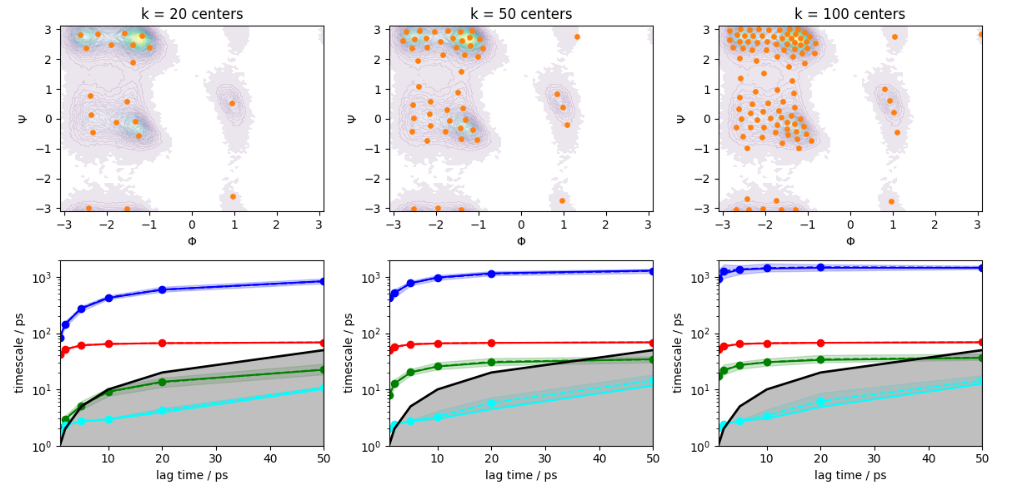
\includegraphics[scale=0.55]{impied.png}
\caption{聚类结果}
\end{figure}


	\subsection{丙氨酸二肽有3个最慢的构象转变过程}





\section{实验方法}
	\subsection{分子动力学模拟}

该研究选取了丙氨酸二肽作为研究对象,选取该分子的原因在于它的结构十分简单,同时该分子已经被充分研究,具有正确的先验知识。在本研究中使用gromacs2021进行分子动力学模拟计算,力场为Amber03,在300K温度下模拟250ns,其中水模型为TIP3P。

	\subsection{马尔可夫模型构建}
构建马尔可夫模型使用了PyEMMA库,使用报道过的方法,首先对轨迹进行了均方根误差(RMSD)计算 ,确认体系达到平衡;随后使用 K-Medoids算法以二面角根据对构象进行聚类,聚类中心为200。

\section{讨论}



\end{CJK}
\end{document}